\documentclass{article}
\usepackage[utf8]{inputenc}
\usepackage[dutch]{babel}
\usepackage[backend=bibtex]{biblatex}
\bibliography{biblatex_DAV.bib}


\title{Oorzaken en Gevolgen van Voedsel-Prijsstijgingen in Niet-Westerse Landen}
\author{Jardenna, Janne, Jonne, Julius}
\date{June 2018}
\usepackage{graphicx} %package to manage images
\graphicspath{ {./images/} }
%Data Analysis and Visualization



\begin{document}


\maketitle

\section*{Inleiding}
% Toen de VOC in de 16e eeuw kruiden en specerijen met de rest van de wereld begon te verhandelen werd een nieuw tijdperk ingeluid. Steeds meer landen volgden het Nederlandse voorbeeld en begonnen handel met elkaar te drijven. Zo ontstond langzaam maar zeker de huidige wereldmarkt waar de prijs van voedselproducten wordt bepaald vraag en aanbood over de gehele wereld.\\

De groei van de internationale heeft er in het algemeen voor gezorgd dat meer landen toegang hebben tot meer buitenlandse producten. Maar het zorgde ook voor meer afhankelijkheid tussen landen, zoals duidelijk werd tijdens de wereldwijde voedselcrisis in 2007. Van veel breed-geconsumeerde producten stegen de prijzen in korte tijd onvoorspelbaar hoog. Zo steeg de wereldwijde prijs van rijst binnen twee jaar met  217\% en de prijs van graan met 136\% \cite{steinberg2008financial}. Hoewel dit ook in ontwikkelde landen voor veel economische en sociale onrust zorgde, bleken hierdoor vooral de ontwikkelingslanden nog armer te worden \cite{ivanic2008implications}. \\

Daarom is er veel onderzoek gedaan naar mogelijke oorzaken van prijsstijgingen, met als doel een herhaling van de voedselcrisis te voorkomen. Zo blijkt het toenemende gebruik van biobrandstoffen de voedselprijzen te verhogen, omdat gewassen worden gebruikt voor het produceren van brandstoffen in plaats van voor de productie van voedsel \cite{mitchell2008note}.
Ook blijkt dat de olieprijs positief gecorreleerd is aan voedselprijzen, omdat het zowel de energiebron is voor mechanische voedselproductie als voor het transporteren ervan\cite{zubrin2008food}. Bovendien vergroot een stijging van de olieprijs weer de vraag naar biobrandstoffen.\\

% Hier wordt met behulp van verschillende data-sets getracht deze mogelijke oorzaken te bevestigen, wat leidt tot de volgende deelvragen:\\
% - Bestaat er een verband tussen de olieprijs en voedselprijzen? \\
% - Bestaat er een verband tussen het bio-brandstofgebruik en voedselprijzen? \\
% Er wordt een positieve correlatie verwacht tussen de olieprijs en alle voedselproducten. Dit is aannemelijk omdat vrijwel alle voedselproducten transport vereisen en hun prijzen daarom afhankelijk zijn van de olieprijs.
% Bovendien wordt verwacht dat de het bio-brandstofgebruik en de prijzen van mais positief gecorreleerd zijn, omdat mais één van de meest populaire gewassen voor bio-brandstof is [Bron]. \\

Naast brandstofgebruik en olieprijzen kunnen echter nog meer factoren in verband staan met fluctuaties van voedselprijzen, zoals geografische factoren. Daaruit volgt de volgende deelvraag:\\
- Vertonen landen in dezelfde regio’s vergelijkbare prijsverschillen? \\
% - Bestaat er een verband tussen regenval en voedselprijzen? \\
Er wordt vanuit gegaan dat landen in dezelfde sub-regio 's soortgelijke fluctuaties in voedselprijzen laten zien, omdat deze landen dikwijls over dezelfde gewassen beschikken en een gelijksoortig klimaat kennen. Hier wordt dat onderzocht door met K-means  verschillende landen bij elkaar te clusteren. Verwacht wordt dat landen in dezelfde regio's significant vaker bij elkaar geclusterd worden, terwijl het clusteren van landen binnen één regio geen vaste cluster-groepen oplevert.  \\
%En dat lange periodes van droogte leiden tot prijsstijgingen van producten zoals rijst en graan. \\

\newpage
Daarnaast bestaan voedselproducten vaak uit dezelfde of gelijksoortige ingrediënten. Daarom wordt ook geprobeerd de volgende deelvragen te beantwoorden:\\
- zijn er voedselprijzen die positief of negatief aan elkaar gecorreleerd zijn? \\
- Als voedselprijzen aan elkaar gecorreleerd zijn, is dit dan altijd het geval of alleen tijdens bepaalde periodes?\\
- Vertonen voedselproducten dezelfde prijsverandering als de ingrediënten waaruit het product bestaat?\\
Er wordt verondersteld dat soortgelijke producten soortgelijke prijsfluctuaties doormaken, en dat de prijsfluctuatie van een voedselproduct dat uit meerdere ingrediënten bestaat overeenkomt met de prijsfluctuaties van die individuele ingrediënten waaruit dat product bestaat. Hier wordt dat onderzocht door de prijzen van zuivelproducten met elkaar te vergelijken, en door de prijzen van brood en de losse ingrediënten van brood met elkaar te vergelijken.
Er wordt verwacht dat de prijzen van zuivelproducten sterk correleren. Deze producten worden immers allemaal van melk gemaakt, en de beschikbaarheid van melk heeft dus waarschijnlijk invloed op de prijzen van al deze producten. Wel wordt verwacht dat deze correlatie niet altijd even sterk is, omdat de beschikbaarheid van andere ingrediënten ook van invloed kan zijn op de prijs.
Bovendien wordt verwacht dat brood dezelfde prijsveranderingen doormaakt als graan, melk en suiker. \\

Bovendien bestaan er vaak ook grote verschillen in welvaart tussen landen. Dat leidt tot de volgende deelvraag:\\
- Kunnen op US-Dollar genormaliseerde prijzen worden gebruikt om de betaalbaarheid van producten te bepalen, of moet er ook gecorrigeerd worden op het Gross Domestic Product (GDP) van een land? \\
Er wordt vanuit gegaan dat corrigeren GDP een betrouwbaarder beeld geeft. Immers kan de GDP tussen landen dermate verschillen dat landen die qua prijsfluctuatie in US-dollars gelijk opgaan, na correctie op GDP geheel andere trends laten zien.
Hier wordt dat onderzocht door van verschillende landen de voedselprijzen in US-Dollar te bepalen, en deze landen met K-means te laten clusteren tot twee groepen met relatief goedkope en relatief dure rijst-prijzen. Vervolgens is dit voor alle landen herhaald, maar dan met prijzen gecorrigeerd op GDP.
Verwacht wordt dat sommigen landen met een laag GDP die met de eerste methode nog tot het goedkope cluster worden gerekend, met de tweede methode in het duurdere cluster worden ingedeeld.\\

Tot slot wordt de beschikbaarheid van voedsel ook vaak in verband gebracht met gezondheid, daarom worden ook geprobeerd de volgende deelvragen te beantwoorden:\\
- bestaat er een verband tussen de voedselprijzen en het sterftecijfer in een land?\\
- bestaat er een verband tussen vluchtelingen-stromingen en voedselprijzen? \\
Er wordt vanuit gegaan dat hoge voedselprijzen een negatieve invloed hebben op de gezondheid, en dat hoge voedselprijzen het aantrekkelijker maakt voor mensen om naar een ander land te vluchten.
Hier wordt dat onderzocht door voedselprijzen met sterftecijfers en vluchtelingen-cijfers te vergelijken.
Verwacht wordt dat er een positief verband bestaat tussen de vluchtelingenstromen, sterftecijfers voedselprijzen. \\

Om deze deelvragen te kunnen beantwoorden is gebruikt gemaakt van de Global Food Prices Database (GFPD) van het World Food Programma (http://www1.wfp.org/). In de database zijn voor 76 verschillende landen de maandelijkse voedselprijzen gegeven voor veel geconsumeerde voedsel waren zoals bonen, rijst en olie. Deze database is uitgebreid genormaliseerd zodat zowel de voedselprijzen van verschillende producten met elkaar vergeleken konden worden als de prijsveranderingen tussen landen en gebieden. \\



\section*{Methode}

\subsection*{Pre-processing}
Ten eerste zijn het is het aantal kolommen van de dataset verminderd. De kolom met de provincies is verwijderd omdat bij het merendeel van de provincies enkel data was verzameld van één stad, waardoor deze kolom geen extra informatie bevatte dan de kolom met steden zelf. Ook waren in de oorspronkelijke dataset de jaren en de maanden gegeven in aparte kolommen. Deze zijn samengevoegd tot één kolom.\\

Vervolgens zijn identieke stads-namen die bij verschillende landen hoorden gedisambigueerd door de afkorting van het betreffende land erachter te zetten. Zo werd San Vicente veranderd naar Sante Vicente (Sal).  Dit was wenselijk omdat er later bij de visualisatie per stad data opgevraagd zou worden. \\
 
Daarna zijn alle eenheden genormaliseerd. Daarvoor zijn alle gewichten naar kilogram (KG) omgezet en alle volumes naar liter (L). Zo was bijvoorbeeld de graanprijs zowel per 1,5 KG als per KG gegeven. Ook dit zou het vergelijken van productprijzen later vergemakkelijken. Bij eenheden waarvoor geen vaste conversion-rate gevonden kon worden zijn de betreffende rijen verwijderd, zoals bijvoorbeeld ‘quartillas’ en (goat) ‘heads’.\\

Ook  zijn alle wisselkoersen en de bijbehorende prijzen genormaliseerd naar US Dollars (USD). Hiervoor is gebruik gemaakt van de .... dataset. Rijen met munteenheden waarvoor geen officiële wisselkoers kon worden gevonden zijn verwijderd. Zo bleek de Somaliland Shilling (SOS)  geen officieel erkende munteenheid te zijn en was er voor de Armenian Dram (AMD) pas wisselkoers-informatie beschikbaar vanaf februari 2003. Alle rijen waar de prijs in SOS was gegeven zijn dus verwijderd, en alle rijen waar de prijs in AMD gegeven was vóór februari 2003 ook.\\

Omdat nu alle prijzen in USD waren gegeven was het ook mogelijk prijzen te normaliseren op koopkracht (GDP) met behulp van de … dataset. Door telkens de GDP van het land door de betreffende prijs van het product te delen ontstond een maat die aangeeft hoeveel er van dat product in het betreffende land gekocht kan worden; hoe hoger het getal hoe beter dat product dus beschikbaar is voor de inwoners van dat land. \\

En omdat het uiteindelijke doel het vergelijken van verschillende voedsel-prijs-grafieken was, en er hiervoor onafgebroken grafieken nodig zijn, zijn alle producten waarvan er meer dan twee opeenvolgende maanden aan data misten verwijderd. Gaps van één of twee jaar zijn ingevuld met behulp van lineaire regressie, waarbij alleen de eerste productprijs vóór en de eerste productprijs ná de gap als referentiepunten zijn gebruikt. \\

Tot slot is voor elke productprijs de afgeleide bepaald zodat de daadwerkelijke veranderingen in voedselprijzen tussen steden en landen vergeleken konden worden, en is met behulp van de … dataset elk land ingedeeld in sub-regio’s zodat ook de voedselprijzen tussen gebieden zoals Midden-Oosten en Indo-China vergeleken konden worden.\\

\subsection*{Exploratory Data Analysis}

\begin{figure}[h]
\centering
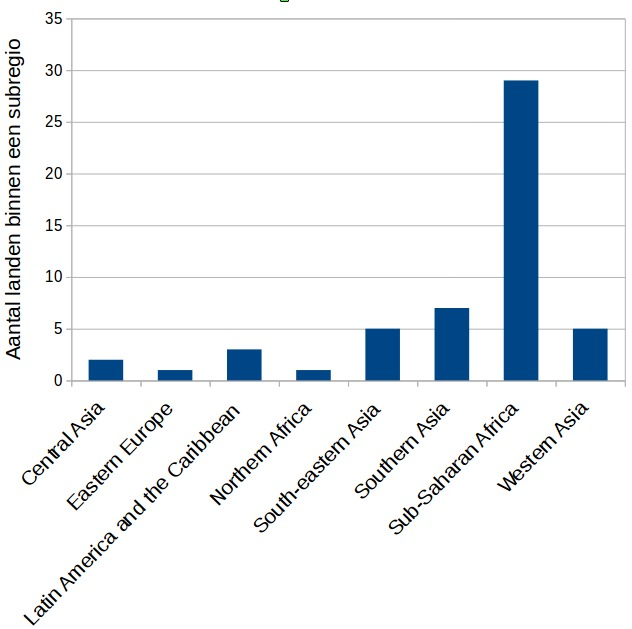
\includegraphics[scale=0.3]{EDA_1}
\caption{het aantal landen per sub-regio }
\medskip
\small
De Sub-Sahara blijkt het meeste landen over te hebben na pre-processing.  
\end{figure}




\subsection*{K-Means Algoritme}
Vervolgens is er een K-Means algoritme geïmplementeerd zodat producten met gelijke prijsveranderingen automatisch bij elkaar gegroepeerd kunnen worden. Dat gebeurt door willekeurig een door de gebruiker gekozen aantal cluster te initiëren en vervolgens elk data-punt toe te wijzen aan het cluster met de kleinste euclidische afstand tot dat punt. 
En door vervolgens in elk cluster alle data-punten bij elkaar op te tellen en de nieuwe cluster-centra op het resulterende gemiddelde te plaatsen, kan het proces van het toewijzen van data-punten aan clusters en het opnieuw berekenen van cluster centra 
iteratief worden herhaald tot de totale euclidische afstand van alle data-punten tot hun cluster-centrum niet of nauwelijks meer afneemt. 

\subsection*{Data-Analyse}
\subsubsection*{verband olie - en voedselprijzen}
Om het verband tussen de olieprijs en de voedselprijzen in Oost-Europa na te gaan is de correlatiecoëfficiënt berekend tussen fluctuaties van de olieprijs en de prijs van 25 verschillende voedselproducten in Oost-Europa, zoals brood melk en eieren.
Daarnaast is zowel de gradiënt van de olieprijs als die van de broodprijs bepaald voor de periode 2013-2018.
In Zuid-Azië is de gradiënt van de olieprijs met de gradiënt van de thee-prijs vergeleken.\\
Vervolgens zijn binnen beide werelddelen de gradiënten met elkaar vergeleken en is de correlatiecoëfficiënt berekend met behulp van...
Tot slot is voor Oost-Europa de correlatiecoëfficiënt tussen de olieprijs en alle andere voedselproducten berekend.


\subsubsection*{Vertonen landen in dezelfde regio’s vergelijkbare prijsverschillen?}
Hiervoor zijn de voedselprijzen binnen de Sub-Sahara vergeleken, omdat dat de regio was met het meeste aantal gedocumenteerde landen in de dataset. Zo konden er meer prijsvergelijkingen gemaakt worden.
Hiervoor zijn voor elke combinatie van twee landen de correlatiecoëfficiënt tussen de rijst-prijzen berekend. Hetzelfde is gedaan voor de kafferkoor-prijzen (een Afrikaans alternatief voor mais). 


\subsubsection*{Kunnen op US-Dollar genormaliseerde prijzen worden gebruikt om de betaalbaarheid van producten te bepalen, of moet er ook gecorrigeerd worden op het Gross Domestic Product (GDP) van een land?}
Hiervoor zijn de genormaliseerde graanprijzen van alle landen in de dataset opgehaald. Hier is voor de graanprijs gekozen omdat graan één van de meest-gedocumenteerde producten in de dataset was (zie figuur 1), waardoor er zoveel mogelijk landen met elkaar vergeleken konden worden. Daarna zijn alle landen met K-means in twee groepen ingedeeld.
Vervolgens is voor elk land de betaalbaarheid-index van graan opgehaald, en zijn op basis hiervan opnieuw met K-means alle landen ingedeeld.

\newpage
\section*{Resultaten}

\subsubsection*{Kunnen op US-Dollar genormaliseerde prijzen worden gebruikt om de betaalbaarheid van producten te bepalen, of moet er ook gecorrigeerd worden op het Gross Domestic Product (GDP) van een land?}

    Met de graanprijs genormaliseerd op US-Dollars, vertonen India, Pakistan en Nepal gelijkmatige graanprijs-fluctuaties. Deze drie landen worden door K-means dan ook samen geclassificeerd tot het cluster met relatief goedkope graanprijzen, terwijl Afghanistan wordt geclassificeerd tot het cluster waar de prijzen hoger liggen. 
     Echter, wanneer er genormaliseerd wordt op GDP, vertoont de grafiek andere fluctuaties. Zo wordt Afghanistan nu samen met Nepal tot het cluster met minder betaalbare graanprijzen geclassificeerd.
 
 
        \begin{figure}[h]
        \centering
        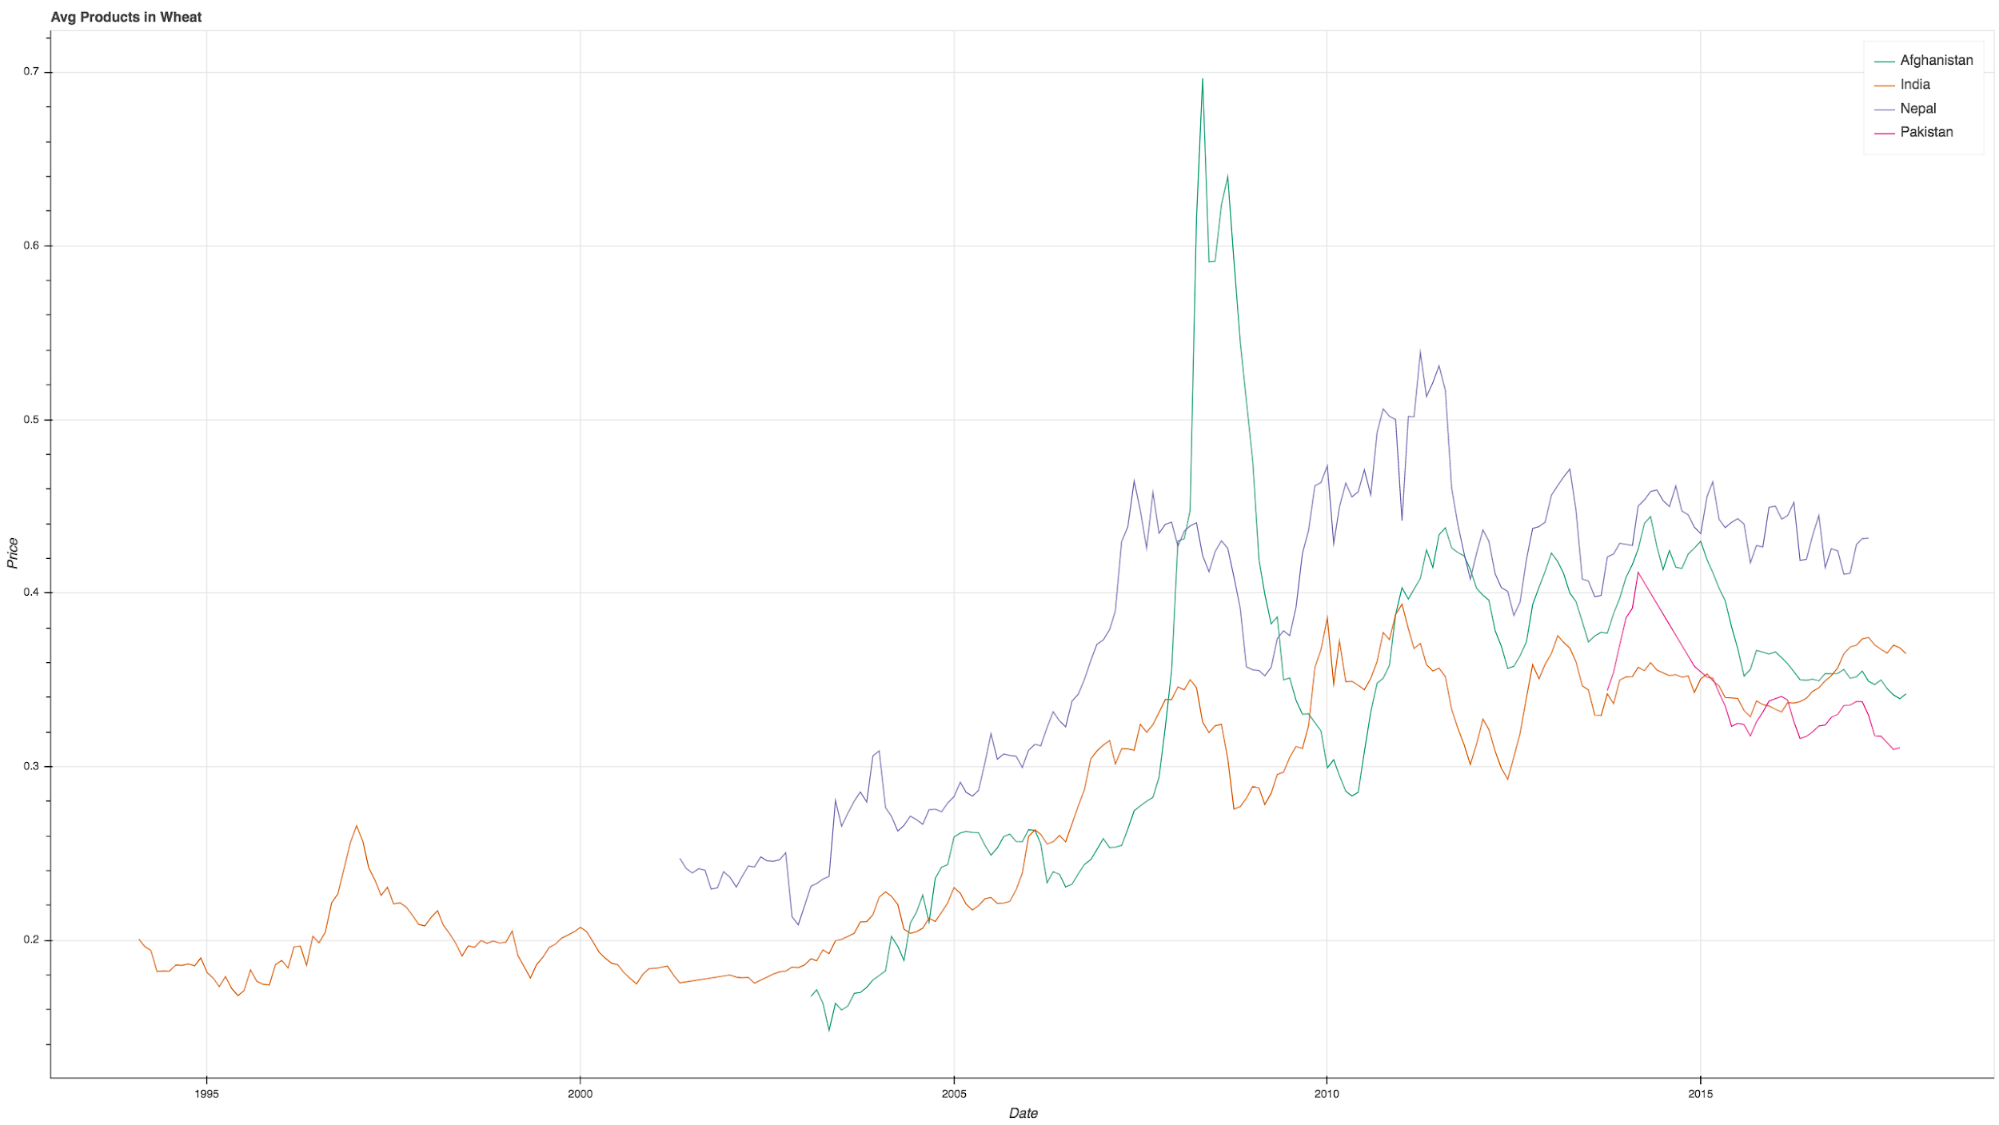
\includegraphics[scale=0.2]{image11.png}
        \caption{De betaalbaarheid van graan over de tijd, zoals gegeven door de absolute prijs in US-Dollar prijzen?}
        \medskip
        \small
        India, Pakistan en Nepal door het K-means algoritme geclassificeerd tot het cluster met relatief goedkopere graanprijzen.  
        \end{figure}
        
        \begin{figure}[h]
        \centering
        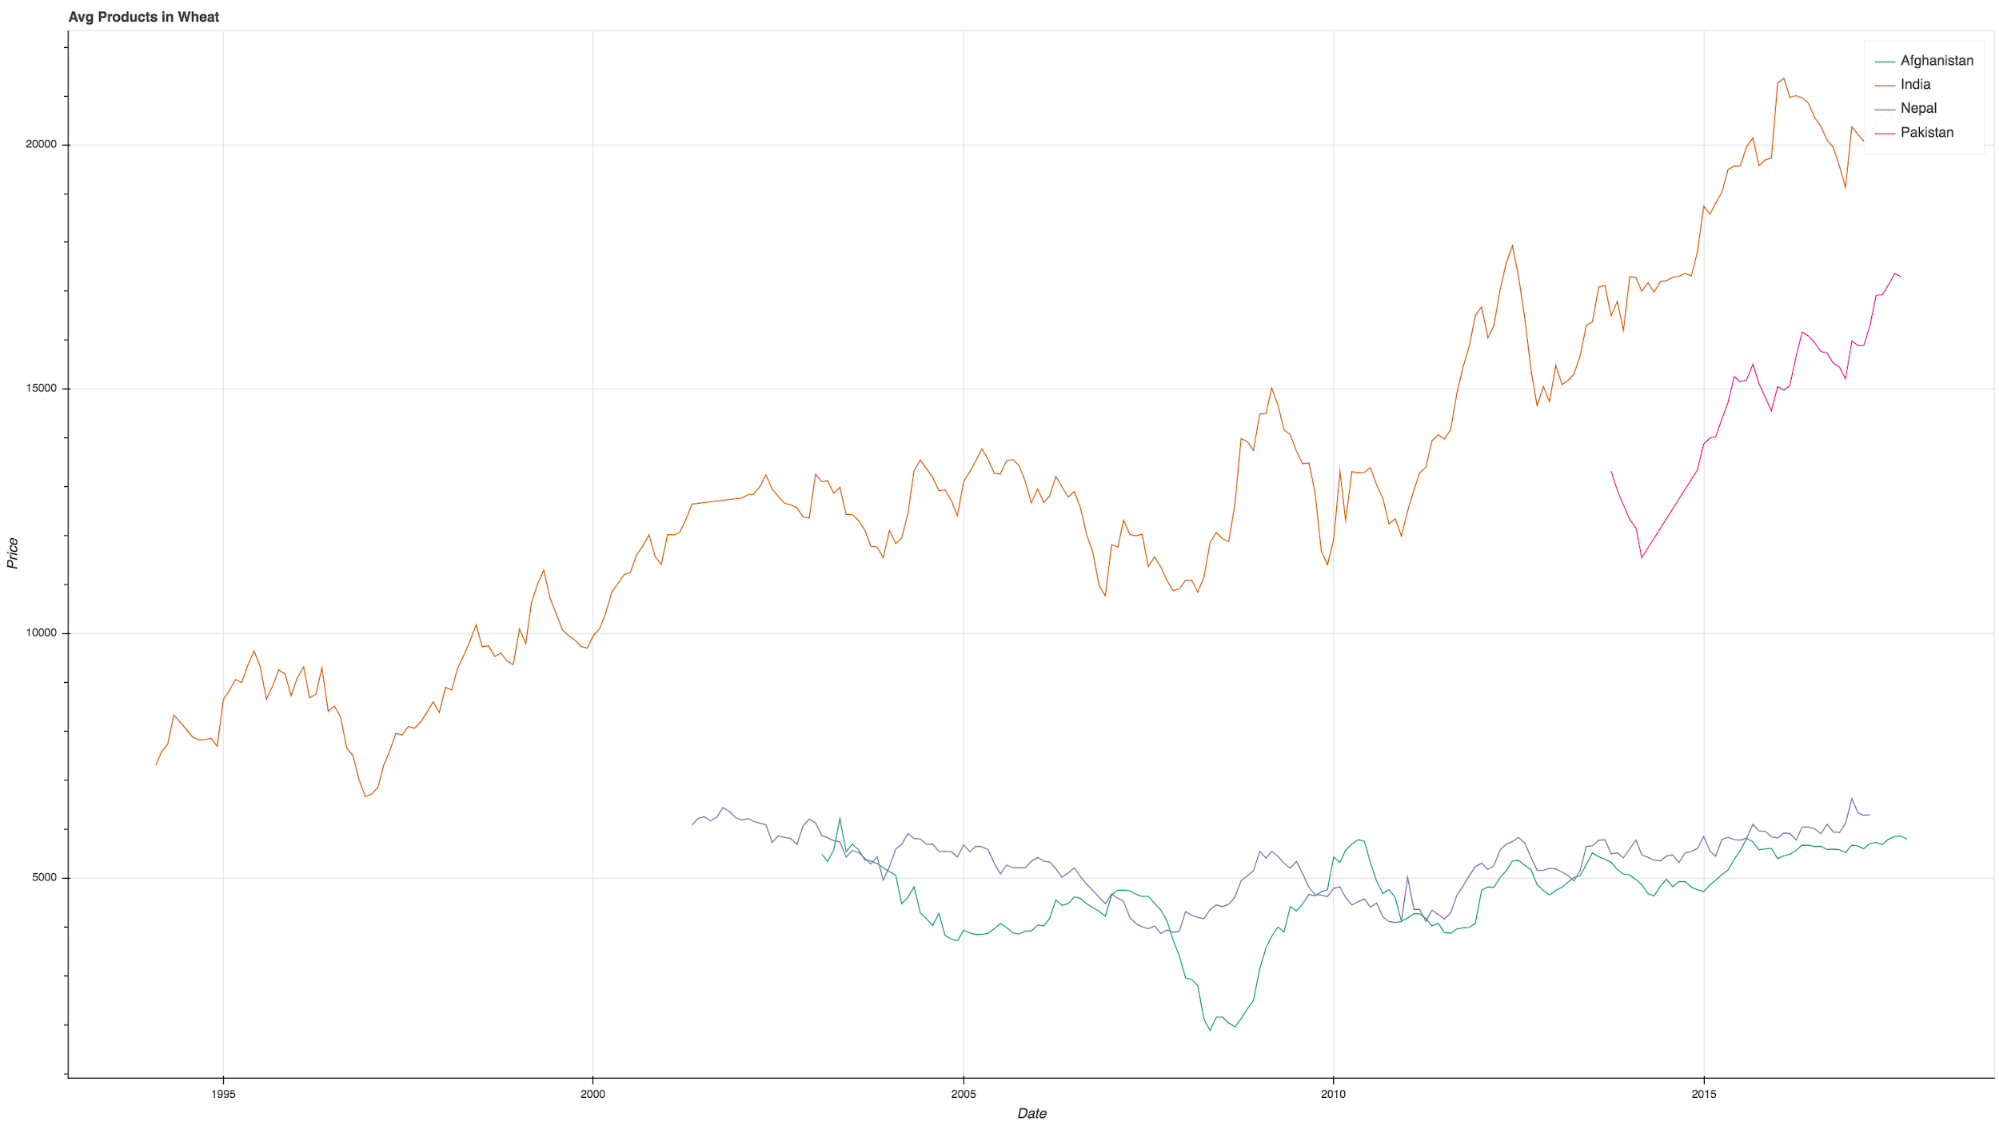
\includegraphics[scale=0.2]{image3.png}
        \caption{De betaalbaarheid van graan over de tijd, gecorrigeerd op GDP}
        \medskip
        \small
        India en Pakistan door het K-means algoritme geclassificeerd tot het cluster met relatief goedkopere graanprijzen, terwijl Afghanistan en Nepal tot het cluster met duurdere prijzen worden gerekend.  
        \end{figure}


 




\newpage

\printbibliography


\end{document}
